\documentclass[12pt]{rapportECL}
\usepackage{lipsum}
\usepackage{fancybox}
\usepackage{float}
\usepackage{amsbsy}
\usepackage{amssymb}
\usepackage{listings}
\usepackage{stmaryrd}
\title{rapport\_tp1} %Titre du fichier
\renewcommand{\thesection}{\arabic{section}} 
\newcommand{\fact}[1]{#1\mathpunct{}!}

\begin{document}

%----------- Informations du rapport ---------

\titre{Reformulation des besoins} %Titre du fichier .pdf
%\UE{UE PRO} %Nom de la UE
%\sujet{\LaTeX Approfondi} %Nom du sujet

\enseignant{
	Renaud \textsc{Vérin}
} %Nom de l'enseignant

\eleves{
	\textsc{BURIE} Aurélien \\
	\textsc{LAFAGE} Adrien \\
	\textsc{LEROUX} Louis-Clément \\
	\textsc{PARAU} Emmanuel
} %Nom des élèves

%----------- Initialisation -------------------
        
\fairemarges %Afficher les marges
\fairepagedegarde %Créer la page de garde
\setcounter{page}{1}

%------------ Corps du rapport ----------------

\section{Introduction}

L'objectif de ce rapport est de vous présenter la façon dont nous avons modlisé les données fournies par le client VDSA. En effet, on nous a fourni un tableau contenant l'ensemble des données concernant les clients de l'entreprise. Nous avons donc créé pour cela plusieurs entités dont les relations vous seront explicités par le biais d'un modèle conceptuel et d'un modèle logique de nos données. Finalement, vous trouverez le code SQL correspondant. 

\tabledematieres %Créer la table de matières
\section{Objectifs :}

Formulation du besoin sous forme de bête à cornes :
\begin{figure}[h]
	\begin{center}
		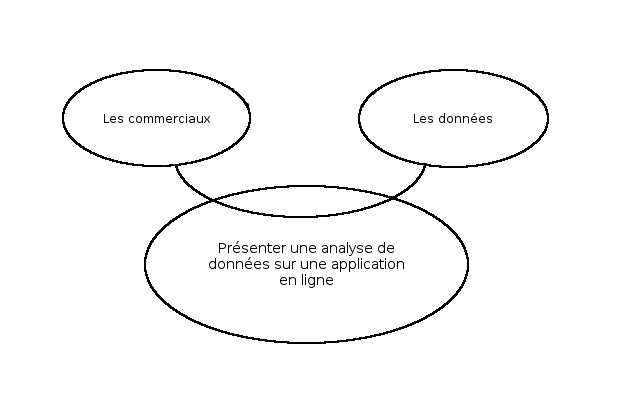
\includegraphics[scale=0.5]{img/beteCornes.png}
		\caption{Bête à cornes}
	\end{center}
\end{figure}

En partant du cahier des charges nous avons réalisé une première liste des fonctionnalités à implémenter sur notre application :

\paragraph{Partie utilisateur :}
\begin{enumerate}
\item[•] Page d'accès au site : doit comprendre une page de connexion avec un mail et un mot de passe, ainsi qu'une option pour faire une demande d'accès auprès de l'administrateurs.
\item[•] Tableau de bord : page principale du site. L'utilisateur doit être redirigé vers cette page après la connexion. Cette page doit contenir tous les graphiques et statistiques nécessaires à l'utilisateur. C'est ici que l'utilisateur doit pouvoir trouver toutes les informations que nous avons extraites de la base de données. De plus, il y aura sur cette page un lien vers la page de géolocalisation.
\item[•] Page de Géolocalisation : sur cette page l'utilisateur devra pouvoir observer comment se répartissent dans l'espace les données fournies par le tableau de bord. Elle contiendra donc une carte Google Map et affichera des zones de couleurs en fonction de critères choisis par l'utilisateur (chiffre d'affaires, marges, ...).
\item[•] Page d'aide : contient tout simplement le manuel d'utilisation de l'application.
\end{enumerate}

\paragraph{Partie administrateur :} La partie administrateur permettra de gérer l'ensemble du site. Les données ainsi que les utilisateurs doivent être validés par l'administrateur. Nous appelerons cette partie de notre site le Back-office. Celui devra permettre :
\begin{enumerate}
\item[•] Le téléchargement de fichiers pour alimenter la base de données.
\item[•] La gestion des comptes utilisateurs.
\end{enumerate}
\clearpage
\section{Objets :}

Du précédent tableau fonctionnel, nous avons extrait l'arborescence technique suivante :
\begin{figure}[h]
	\begin{center}
		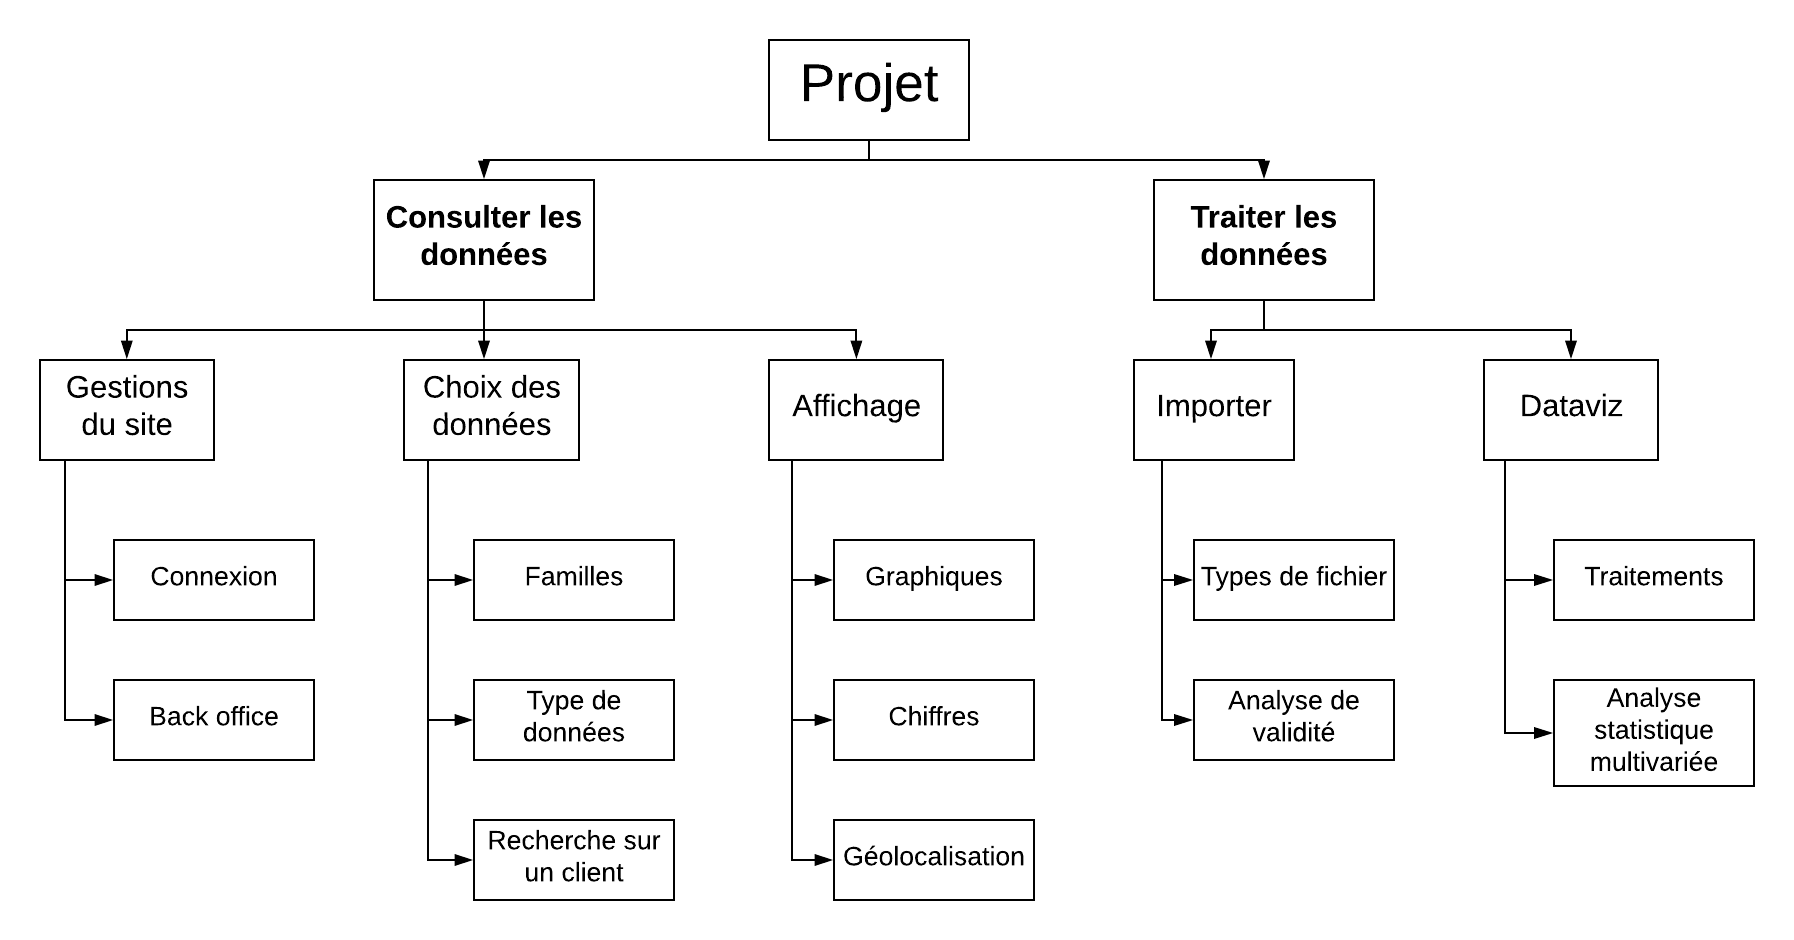
\includegraphics[scale=0.6]{img/ArborescenceTechnique.png}
		\caption{Arborescence technique}
	\end{center}
\end{figure}
%\clearpage
%\input{operations.tex}
\clearpage
\section{Opérations et Ordre :}

\begin{figure}[h]
	\begin{center}
		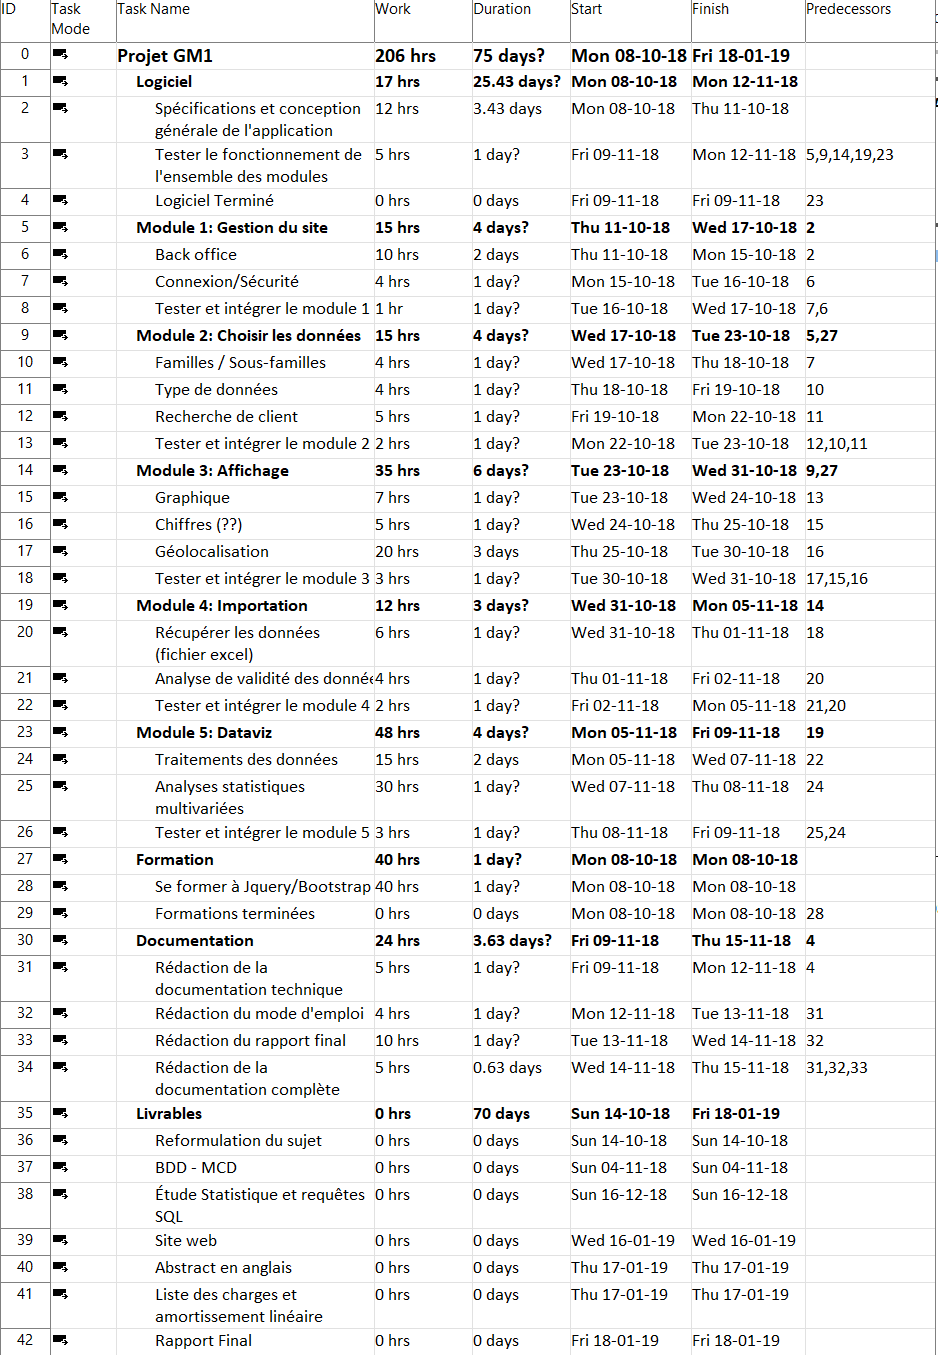
\includegraphics[scale=0.6]{img/planning.png}
		\caption{Planning}
	\end{center}
\end{figure}
\clearpage
\section{Opérateurs :}
\clearpage
\section{Outils :}

Nous présenterons ici nos outils de développement et de gestion du projet. Concernant l'implémentation de l'application nous utiliserons les langages suivants :\\
\begin{enumerate}
\item[•] Côté serveur : PHP (contrainte donnée par les consignes de réalisation)
\item[•] Côté client : Html, Css et Javascript
\end{enumerate}
Dans le but d'accélérer notre producivité dans la réalisation du css et du javascript, nous utiliserons les frameworks : Bootstrap et jQuery.\\

Par ailleurs, nous avons choisi d'utiliser la plateforme de versionning : GitHub, afin de pouvoir travailler à plusieurs et de façon claire sur le code. De plus, il possèdera de la documentation rédigée en Markdown.

%------------ Fin du document  -----------------
\end{document}

%https://openclassrooms.com/forum/sujet/formulaire-de-formules-latex-84687
